\documentclass{article}
\usepackage{arxiv}
\usepackage[utf8]{inputenc} % allow utf-8 input
\usepackage[T1]{fontenc}    % use 8-bit T1 fonts
\usepackage{hyperref}       % hyperlinks
\usepackage{url}            % simple URL typesetting
\usepackage{booktabs}       % professional-quality tables
\usepackage{amsfonts}       % blackboard math symbols
\usepackage{nicefrac}       % compact symbols for 1/2, etc.
\usepackage{microtype}      % micro typography
\usepackage{graphicx}
\usepackage{subcaption}
\usepackage[scaled]{beramono}
\usepackage[procnames]{listings}
\usepackage{color}
\usepackage{wrapfig}
\usepackage[toc,page]{appendix}
\usepackage{import}
\usepackage{verbatim}

\definecolor{keywords}{RGB}{255,0,90}
\definecolor{comments}{RGB}{0,0,113}
\definecolor{red}{RGB}{160,0,0}
\definecolor{green}{RGB}{0,150,0}
\DeclareUnicodeCharacter{3C9}{ }
\raggedbottom

\newcommand{\code}[2]{
    \hrulefill
    \subsection*{#1}
    \lstinputlisting[
        language=Python,
        basicstyle=\ttfamily\small,
        keywordstyle=\color{keywords},
        commentstyle=\color{comments},
        stringstyle=\color{red},
        breaklines=true,
        showstringspaces=false,
        numbers=left,
        stepnumber=1,
        procnamekeys={def,class}
    ]{#2}
    \vspace{2em}
}

\newcommand{\logoutput}[2]{
    \hrulefill
    \subsection*{#1}
    \lstinputlisting[
        language=Python,
        basicstyle=\ttfamily\small,
        commentstyle=\color{comments},
        stringstyle=\color{red},
        breaklines=true,
        showstringspaces=false,
        numbers=left,
        stepnumber=1,
        procnamekeys={Query variable,Evidence,Ordering}
    ]{#2}
    \vspace{2em}
}

\title{Human-Robot Interaction}
\renewcommand{\undertitle}{Robot learning}
\date{}

\author{
    J. Verhaert \\
    S1047220\\
    Master Artificial Intelligence | Intelligent Technology \\
    \texttt{joost.verhaert@student.ru.nl} \\
    \And
    T. Gelton \\
    S4480783\\
    Master Artificial Intelligence | Intelligent Technology \\
    \texttt{thijs.gelton@student.ru.nl} \\
}
\renewcommand{\headeright}{Robot learning}

\begin{document}
    \maketitle
    \pagebreak


    \section{Introduction}\label{sec:introduction}
    %- Describe the stages for completing the task
    The goal of the second assignment of Human-Robot Interaction is to incorporate robot learning techniques in HRI applications. Part one of this assignment gives a brief introduction about the concepts and techniques (e.g. using derivatives in backpropagation) needed for deep learning. Last year, both of us followed the Neural Network course during our pre-master, but it was still a pleasant refresher. Part two showed the differences between a Feed Forward Network (FFN) and a Mixed Density Network (MDN) and most important how the MDN is able to learn multi-valued mappings. In this study we describe how we applied this new network in order to have Webots' Nao learn the \textit{Inverse Kinematics} of tracking a green ball by hand.

    \section{Methods and algorithms}\label{sec:methods-and-algorithms}
    The two algorithms that were used for the task of robot learning were a FFN and a MDN.
    Regarding the popularity of deep learning, the FFN is widely used and does not need an in\-depth explanation.
    In short, it allows the modelling of non-linear distributions and performs exceptionally well on unstructured data.
    A MDN is a network that allows to make multi-valued predictions.
    Meaning that a learned MDN outputs Gaussians and these are then used to sample from.
    This allows it to model 1\-to\-many relations, where the input has multiple possible outputs.
    Bishop\cite{bishop1994mixture}, shows an inverse sinusoid and how a MDN is able to model this where a FFN is not.
    %- Methods: Explain the methods/algorithms used and explain why

    However, for any algorithm the first step to take is to gather data.
    For this we re-used some of Nao's parts from the first assignment, i.e. the keyboard functionality and the segmentation of the ball in the image.
    In a step-by-step manner, the arm is first moved, then the ball is manually aligned and then the 'E' key is pressed to create a new data point.
    This CSV file is imported into a PyTorch Dataset object (see notebook) and deduplicated to make sure that every X and Y coordinate-pair of the ball only has one corresponding roll ($\theta_1$) and pitch ($\theta_2$) angle.

    After importing the data, which consisted of 72 samples after deduplication, the MDN was trained first.
    For this we used the Adam optimizer and a Negative Log-Likelihood (NNL) loss function.
    The Adam optimizer needed an epsilon of $1e-05$ to compensate for the often occurring vanishing gradient when using the NNL loss function.
    For this very reason, using a train and validation set was infeasible. 
    The size of the dataset strongly impacted this vanishing gradient and thus all samples were needed in order to train the MDN model.   
    Only one sample was reserved for testing.
    The network itself has two inputs that are connected, via 1 hidden layer of 20 nodes, to the pi-($\pi$), sigma-($\sigma$) and mu($\mu$) layer.
    Both the MDN and FFN use Tanh activation functions.
    The number of Gaussians, and thus the number of $\pi$, $\sigma$ and $\mu$ outputs, depends on the domain and it is up to the designer to specify this number.
    In the results (page \ref{sec:results}) section we will compare the differences in the number of Gaussians.

    To be able to compare the FFN and MDN, only one hidden layer with 20 nodes was used for the FFN as well.
    The network was then trained using the Mean Squared Error (MSE) and the same Adam optimizer as with the MDN.

    One possibility with deep neural networks is to have the network extract the ball from an image itself instead of using the distilled coordinates by segmentation. 
    In order to do so, the first layer should be substituted by convolutional layers.
    Another possibility would be to use a pretrained model trained on a large dataset and substitute the final layer to get the output needed.
    This would require some retraining of the weights, but will result in better visual detection.
    For this controlled toy experiment this would not be necessary.


    \section{Results}\label{sec:results}
    %- Describe the results incorporating the advantages and limitations of the methods used.
    \begin{wrapfigure}{l}{0.5\textwidth}
        \begin{center}
          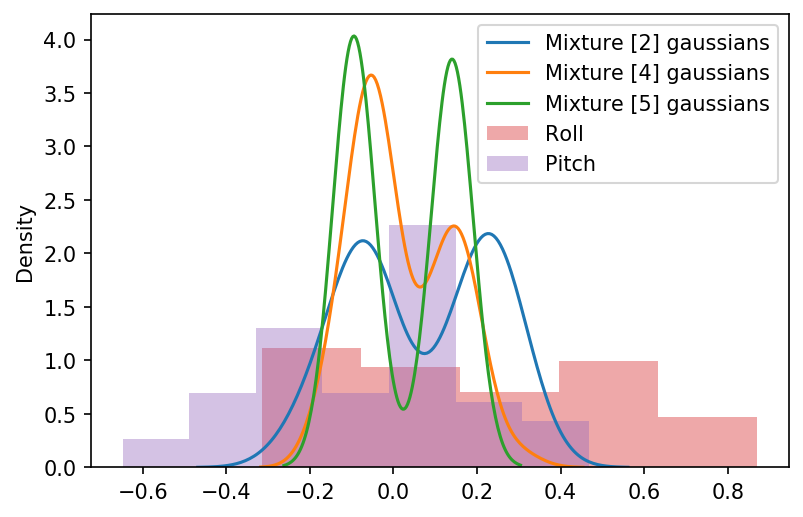
\includegraphics[trim=0 0 0 23pt,width=0.48\textwidth]{../part2/20kepochs_distr.png}
        \end{center}
        \caption{Mixture Models at different number of Gaussians and the target distribution. Input to each model was the mean of the x and y coordinates of the ball.}
        \label{fig:learned-mix-model}
        \vspace{-40pt}
    \end{wrapfigure}

    Eventually we chose to use 2, 4 and 5 gaussians and compare the results.
    The learned distributions can been seen in figure \ref{fig:learned-mix-model}.
    In this specific case, different combinations of $\theta_1$ and $\theta_2$ could not lead to the same position and thus the MDN would quickly converge to a point where the outputted $\pi$ would become a one-hot encoded vector (e.g. [0, 0, 1, 0]). 
    Formulated differently, the model would not be doubting about a multitude of distributions describing the actual distribution best, it would only have to converge to one to best model it. 
    This meant that the Mixture Model would converge to only one Gaussian.
    When inspecting figure \ref{fig:learned-mix-model}, you can clearly see that there are two means for each mixture, one for each output, and that number of gaussians correlate to the size of the covariance.
    It seems that the number of Gaussians gave the model more freedom to become more precise with the distribution as the amount went up.
    I.e., more gaussians meant narrower distributions.


    \begin{figure}[!htb]
        \centering
        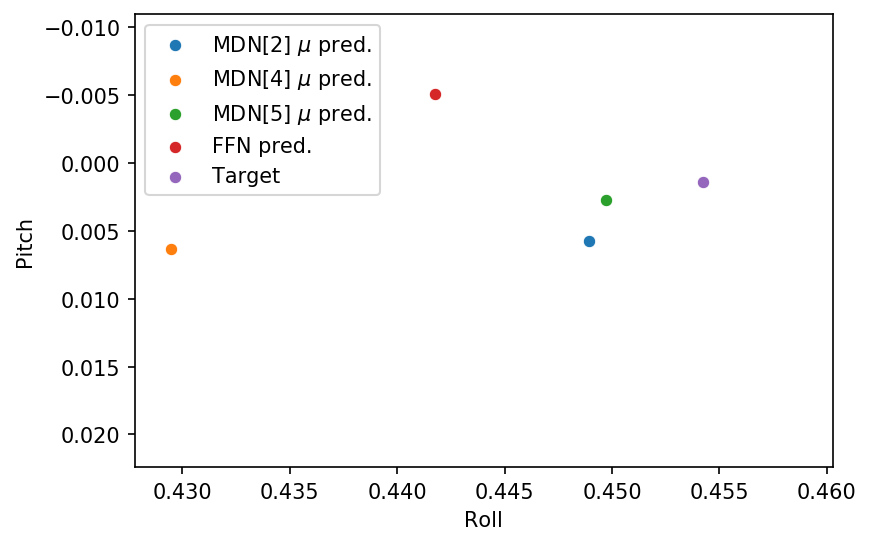
\includegraphics[width=.8\textwidth]{../part2/all_mod_predictions.png}
        \caption{Predictions of the MDN models and the FFN model on the validation sample (N = 1).}
        \label{fig:pred-models}
    \end{figure}

    Aside from inspecting Nao's behavior, the FFN and the different MDN models were tested against the validation sample (N = 1).
    In figure \ref{fig:pred-models} you can see that the best performing model is the MDN with 5 gaussians.
    Do note that this is not representative as it is only 1 sample, but in order to be able to train the MDNs without the vanishing gradient nearly all samples were needed for training.
    On the other hand, this one sample is unseen for all models, which is also important in testing.

    A factor that was impossible to capture by still images, was the actual performance of all models in the simulator.
    Eventually, the FFN seem to outperform the MDNs as the MDN caused some oscillation whereas the FFN tracked the ball in a seemingly precise and smooth manner.
    The MDN with 4 gaussians showed the best tracking capability by a small margin compared to 5 gaussians.

    \section{Conclusion}\label{sec:conclusion}
    %- Draw your own conclusion about this robot learning approach
    There are multiple conclusions to draw from this experiment. First and foremost it is important to state that learning in intelligent systems is indispensable. 
    In order to create an autonomous intelligent system, learning is key ingredient. 
    However, for autonomous learning this present study is inadequate, as this was done in a supervised manner. 
    A robot in an unknown and hostile environment has to be able to orient itself, explore its environment, recover from failures and must generalize well in order to solve a multitude of different tasks\cite{thrun1995lifelong}. 
    
    Still, the difficulty of a task can be seen as a spectrum and each task will have its own solution. 
    For the ball tracking behavior by (Nao's) hand both the models showed promising results. 
    As described in section \ref{sec:results}, the problem at hand only required Nao to use two degrees of freedom to learn the \textit{Inverse Kinematics}.
    Contradictory to the example by Bishop\cite{bishop1994mixture} (which also uses two degrees of freedom), different $\theta_1$ and $\theta_2$ values could not result in the same outcome of the arm.
    Comparing these two models in this study would be senseless as both have their own usefulness and referring back to the beginning of this paragraph: are a solution to a specific task.
    A better use of the MDN is displayed by \cite{mirrazavi2018unified}, where they use two robotic arms that perform under 7 degrees of freedom (DOF) that need to avoid each other while touching an air bound thrown object.
    Here, the MDN is used to compute different \textit{feasible intercept points} for the thrown object in respect to the arm.

    Eventually, even when taking into account that both of us already understood the FFN, the MDN still seemed to be a more difficult concept to grasp and to implement.
    Thus concluding, for this study the FFN would be our model of choice for the problem.
    If the problem would have more degrees of freedom, then the MDN would be the better choice.



    % \cite{mirrazavi2018unified} <-- multi arm motion planning with MDN's. Usable as citation

    \pagebreak
    \bibliographystyle{ieeetr}
    \bibliography{main}
\end{document}
